\section{Пространственная когерентность. Степень пространственной когерентности. Звездный интерферометр Майкельсона и его современные модификации. } 
\subsection{Пространственная когерентность.}

\Def{Пространственная когерентность}  --  когерентность колебаний, которые совершаются в один и тот же момент времени в разных точках плоскости, перпендикулярной направлению распространения волны.
Вводится для объяснения интерференции нескольких источников.
Два источника называются пространственно когерентными, если их размеры и расположение позволяют наблюдать интерференцию.
\begin{theor}\label{2  некогерентных точечных источника.}

Условие для хорошей контрастности интерференционной картины($\alpha$ - правильная дробь):
\begin{equation}
\Delta = l[\cos{\beta_1}-\cos{\beta_2}]=(m+\alpha)\lambda, \alpha \in [0, 1/4]\label{23.1}
\end{equation}

Максимумы и минимумы накладываются:
\begin{equation}
\Delta = l[\cos{\beta_1}-\cos{\beta_2}]=m\lambda \label{23.2}
\end{equation}

Компенсируются:
\begin{equation}
\Delta = l[\cos{\beta_1}-\cos{\beta_2}]=(m+1/2)\lambda\label{23.3}
\end{equation}
\end{theor}
\begin{proofn}
Рассмотрим интерференцию от двух точечных источников A и B. P-точка интерференции. Из точки A исходят два луча: $AM_1P$ и $AM_2P$, которые друг с другом интерферируют в точке P. Аналогично для точки B есть 2 луча $BN_1P$ и $BN_2P$. 
\begin{figure}[H]
\center{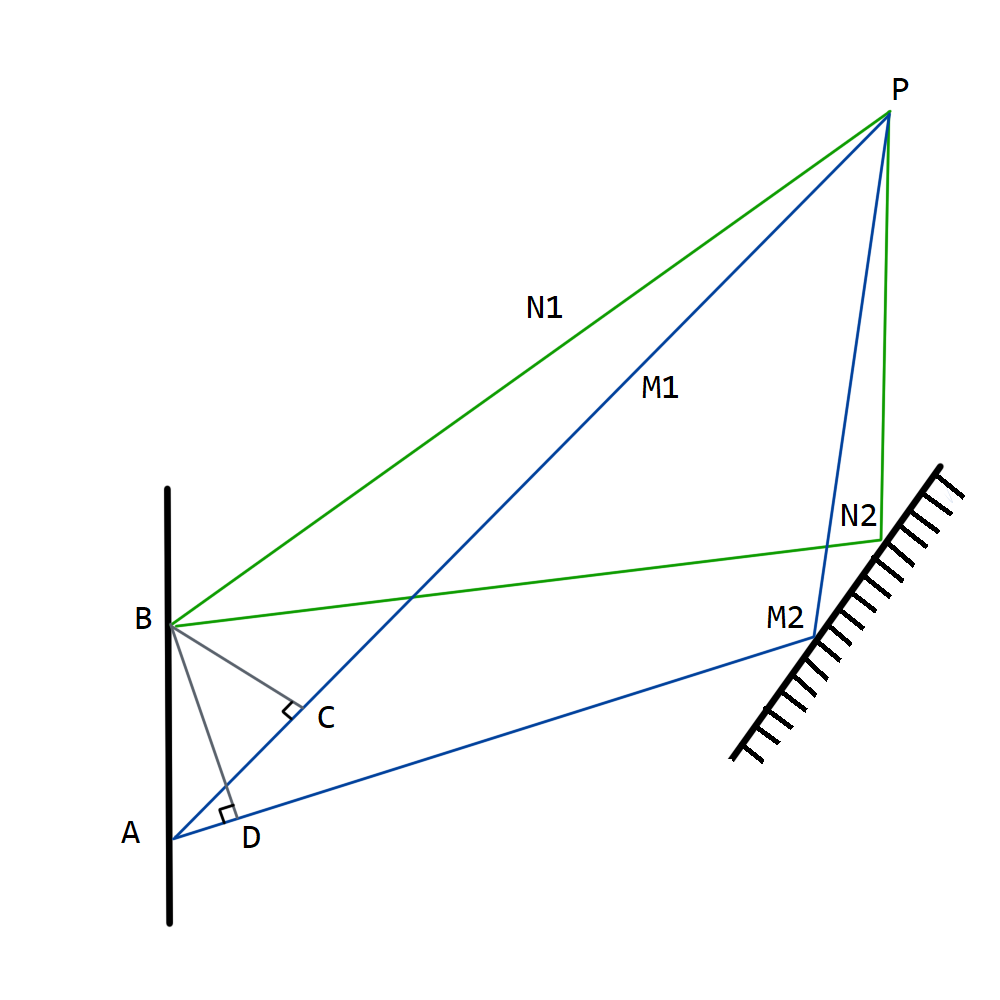
\includegraphics[scale=0.3]{8}}
\end{figure}
Если расстояние $AB=l$ мало, оптическая разность хода лучей от A и B:
$$\Delta_A=(AM_1P)-(BN_1P)=(AC)=\cos{BAC}=\cos{\beta_1}$$
$$\Delta_B=(AM_2P)-(BN_2P)=(AD)=\cos{BAD}=\cos{\beta_2}$$
 И результирующая разность хода:

$\Delta=|\Delta_A-\Delta_B|=l|\cos{\beta_1}-\cos{\beta_2}|$  --характеризует относительный сдвиг двух независимых интерференционных картин

$\Delta \sim 0$ или $\Delta \sim \lambda$, сдвиг нулевой$\qrq$максимумы и минимумы складываются.

$\Delta \sim \lambda$,  максимумы накладываются на минимумы$\qrq$ интерференционная картина пропадает.

Очевидно, при сдвиге на целое число длин волн картина не меняется.
Условие \ref{23.1} отражает промежуточное состояние, может показаться произвольным, но ним так будет удобно в будущем.
\end{proofn}
\begin{theor}\label{Протяженный источник длины l.}
Разобьем источник на пары некогерентных точек $(A_1 B_1), (A_2 B_2), ... $ находящихся на расстоянии l/2. Для каждой из них можно записать условие \ref{23.3}: 
\\$\frac{l}{2}||\cos{\beta_1}-\cos{\beta_2}|=\frac{\lambda}{2}$ или $\delta= l[\cos{\beta_1}-\cos{\beta_2}]=\lambda$ 

То есть каждая пара не дает интерференционных полос$\qrq$мы видим равномерный светлый фон.
Аналогично, если $\delta=(m+\alpha)\lambda$, где $\alpha$ правильная дробь, мы можем разбить источник на две части в пропорции $m:\alpha$. Меньшая часть будет создавать полосы на светлом фоне, создаваемом большей частью. Чем больше m, тем хуже видно интерференцию.

Условие хорошей контрастности:
$\delta= l[\cos{\beta_1}-\cos{\beta_2}]|\leq \lambda/2$
\\Если существует точка, из которой лучи исходят симметрично, т.е $\beta_2=\pi-\beta_1$, угол между этими лучами - угол интерференции $\Omega = \beta_2-\beta_1=\pi - 2\beta_1$.
$$|\cos{\beta_1}-\cos{\beta_2}|=2\cos{\beta_1}=\sin({\frac{\pi}{2}-\beta_1})=\sin{\frac{\Omega}{2}}$$ %РИСУНОК
В этом случае условие хорошей контрастности: 
$ l\frac{\sin{\Omega}}{2}\leq \lambda/4$ 
\end{theor}
\subsection{Степень пространственной когерентности.}
Для определения степени когерентности вообдят понятие 

\Def{Корреляционная функция} -- Зависящая от времени корреляция двух случайных функций $E(r_1, t_1)$ и $E(r_2, t_2)$ определяется как $B(r_1, t1, r_2, t_2)\langle E(r_1, t_1) E(r_2, t_2)\rangle$, где угловые скобки обозначают процедуру усреднения.  

\Def{Степень когерентности}
Для светового пучка введем величину $$\gamma(r_1,r_2, t=t_1-t_2)=\frac{B}{\sqrt{I_1I_2}}$$ -- комплексную степень когерентности. $\gamma\leq1$ 
При t=0 $|\gamma|$ -- степень пространственной когерентности, а при $r_1=r_2$ -- степень временной когерентности.
\subsection{Звездный интерферометр Майкельсона}
Если поставить на пути лучей источника экран с двумя отверстиями, расположенными на расстоянии D, появляется специфицеская картина. Если закрыть одно отверстие, то дифракция лучей на втором даст стандартную картину колец, однако если открыть оба отверстия, две системы колец совместятся. К эффекту обычного сложения минимумов и максимумов добавится интерференция двух щелей и кольца будут пересечены интерференционными полосами. Угловое расстояние между этими полосами определяется угловым расстоянием -- углом, на который отличаются направления на соседние интерференционные максимумы:$\upsilon=\lambda/D$.
Допустим, мы наблюдаем в такую систему двойную звезду с угловым расстоянием $\delta\phi=\upsilon/2$ между ее компонентами. Тогда минимумы интерференционных полос от одной звезды наложатся на минимумы другой. Изменяя расстояние D можно добиться картины, на которой интерференционные полосы пропадут совсем или их видимость станет наименьшей.  В таком случае угловое расстояние между компонентами звезды станет 
$$\delta\phi=\frac{\lambda}{2D}$$
Для одиночной звезды можно применить тот же метод: для упрощения вычислений можно проедполоэить, что звезда излучает как квадрат, плоскоссть которого параллельная фокальной плоскости объектива, а пара сторон параллельная прямой, соеддиняющей отверстия экрана. Тогда можно разбить этот квадрат на пары полосок(аналогично случаю с протяженным источником в этом же билете), каждая пара не даст интерференционных полос. Подобрав D так, что интерференционные полосы исчезнут,угловой размер стороны квадрата можно найти по формуле   $\delta\phi'=\frac{\lambda}{D}$
Если звезду представить как равномерно светящийся диск, угловой размер можно найти по формуле $\delta\phi'=1,22\frac{\lambda}{D}$
Проблема этого метода в том, что для хорошей интерференции нужен телескоп с большим диаметром объектива. Майкельсон соединил телескоп с интерферометром и решил эту проблему, добавив зеркала.
\begin{figure}[H]
\center{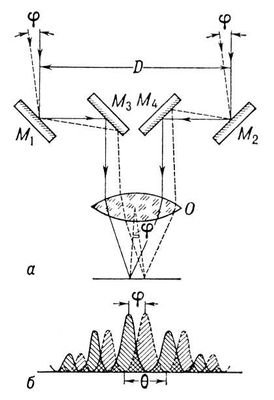
\includegraphics[scale=0.5]{9}}
\end{figure}
Изменяя расстояние между отверстиями и перемещая зеркала, можно добиться исчезновения интерференционной картины.
\subsubsection{Принцип работы звездного интерферометра Майкельсона}
По принципу Гюйгенса-Френеля заменим звезду на вторичный фронт(уберем звезду, поместим вторичные источники $S_1$ и $S_2$ в отверстия экрана.) Зеркала дадут 2 пары мнимых изображений. Если от звезды идет пучок параллельных лучей, то источники, а значит, и их изображения, будут в одной фазе. Получается, что зеркала позволяют "сблизить" вторичные источники, а интерференционная картина сохранится. 

Теперь расположим вторую звезду на расстоянии $\delta\phi$ от первой. Ее волновой фронт будет достигать отверстий не одновременно(нет симметрии) Разность хода между лучами, приходящими в отверстия, будет равна $D\delta\phi$. Интерференционные полосы минимизируются, если разность хода будет равна $D\delta\phi=\lambda/2$. Получилась формула, идентичная старой модели телескопа.

Проблема телескопа такой конструкции в том, что система зеркал  должна быть строго неподвижной и при этом раздвигаться на большое расстояние.
\subsubsection{Современные модификации.}
Я не имею ни малейшего понятия, что тут имеется в виду, но вот что накопалось в гугле:
\begin{figure}[H]
\center{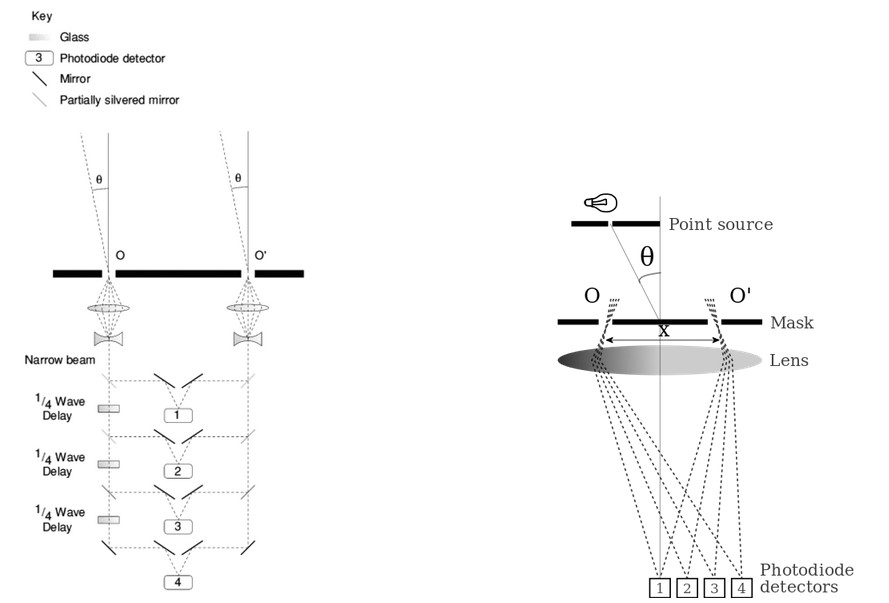
\includegraphics[width=\textwidth]{10}}
\caption{Слева: двухэлементный оптический интерферометр. Справа: Интерферометр с дополнительной диафрагмой.}
\end{figure}
Простой двухэлементный интерферометр устроен следующим образом: Свет от двух телескопов(на схеме изображены как линзы) с помощью системы пластинок и зеркал направляется в 4 независимых детектора. Пластинки обеспечивают фазовую задержку и позволяет измерить видность изображения.
 
В телескопе с диафрагмой используется несколько датчиков, во которые свет будет попадать, пройдя один и тот же оптический путь, что позволяет увеличить точность измерений.